%%
% Modificación de una plantilla de Latex para adaptarla al castellano.
%%

%%%%%%%%%%%%%%%%%%%%%
% Thin Sectioned Essay
% LaTeX Template
% Version 1.0 (3/8/13)
%
% This template has been downloaded from:
% http://www.LaTeXTemplates.com
%
% Original Author:
% Nicolas Diaz (nsdiaz@uc.cl) with extensive modifications by:
% Vel (vel@latextemplates.com)
%
% License:
% CC BY-NC-SA 3.0 (http://creativecommons.org/licenses/by-nc-sa/3.0/)
%
%%%%%%%%%%%%%%%%%%%%%

%----------------------------------------------------------------------------------------
%	PACKAGES AND OTHER DOCUMENT CONFIGURATIONS
%----------------------------------------------------------------------------------------

\documentclass[a4paper, 11pt]{article} % Font size (can be 10pt, 11pt or 12pt) and paper size (remove a4paper for US letter paper)
\usepackage{helvet}
\renewcommand{\familydefault}{\sfdefault}
\usepackage[protrusion=true,expansion=true]{microtype} % Better typography
\usepackage{graphicx} % Required for including pictures
\usepackage[usenames,dvipsnames]{color} % Coloring code
\usepackage{wrapfig} % Allows in-line images
\usepackage[utf8]{inputenc}
\usepackage{enumerate}
\usepackage{enumitem}

% Imágenes
\usepackage{graphicx} 

\usepackage{amsmath}
% para importar svg
%\usepackage[generate=all]{svgfig}

% sudo apt-get install texlive-lang-spanish
\usepackage[spanish]{babel} % English language/hyphenation
\selectlanguage{spanish}
% Hay que pelearse con babel-spanish para el alineamiento del punto decimal
\decimalpoint
\usepackage{dcolumn}
\newcolumntype{d}[1]{D{.}{\esperiod}{#1}}
\makeatletter
\addto\shorthandsspanish{\let\esperiod\es@period@code}
\makeatother

\usepackage{longtable}
\usepackage{tabu}
\usepackage{supertabular}

\usepackage{multicol}
\newsavebox\ltmcbox

% Para algoritmos
\usepackage{algorithm}
\usepackage{algorithmic}
\usepackage{amsthm}

% Para matrices
\usepackage{amsmath}

% Símbolos matemáticos
\usepackage{amssymb}
\usepackage{accents}
\let\oldemptyset\emptyset
\let\emptyset\varnothing

\usepackage[hidelinks]{hyperref}

\usepackage[section]{placeins} % Para gráficas en su sección.
\usepackage[T1]{fontenc} % Required for accented characters
\usepackage{tikz}
\newenvironment{allintypewriter}{\ttfamily}{\par}
\setlength{\parindent}{0pt}
\parskip=8pt
\linespread{1.05} % Change line spacing here, Palatino benefits from a slight increase by default

\makeatletter
\renewcommand\@biblabel[1]{\textbf{#1.}} % Change the square brackets for each bibliography item from '[1]' to '1.'
\renewcommand{\@listI}{\itemsep=0pt} % Reduce the space between items in the itemize and enumerate environments and the bibliography
\newcommand{\imagen}[2]{\begin{center} \includegraphics[width=90mm]{#1} \\#2 \end{center}}
\newcommand{\RFC}[1]{\href{https://www.ietf.org/rfc/rfc#1.txt}{RFC-#1}}

\renewcommand{\maketitle}{ % Customize the title - do not edit title and author name here, see the TITLE block below
\begin{center} % Center align
{\Huge\@title} % Increase the font size of the title
\end{center}

\vspace{20pt} % Some vertical space between the title and author name

\begin{flushright} % Right align
{\large\@author} % Author name
\\\@date % Date

\vspace{40pt} % Some vertical space between the author block and abstract
\end{flushright}
\renewcommand{\baselinestretch}{0.5}

}


\usepackage[a4paper]{geometry}
\geometry{top=2cm, bottom=2cm, left=2.25cm, right=2.25cm}

%----------------------------------------------------------------------------------------
%	TITLE
%----------------------------------------------------------------------------------------

\title{\textbf{Ecuación de la elipse}\\ % Title
\vspace{20 pt}
Mecánica Celeste} % Subtitle

\author{\textsc{Daniel López García\\
Íñigo San Jose Visiers\\
Lothar Soto Palma} % Author
\\{\textit{Universidad de Granada}}} % Institution

\date{\today} % Date

\newcounter{ndef}

\begin{document}
	\maketitle
	\begin{center}
		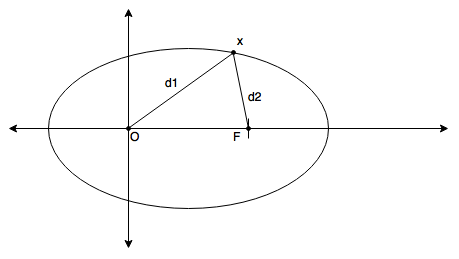
\includegraphics[scale=0.75]{elipse.png} 
	\end{center}	\addtocounter{ndef}{1}
	Consideramos la elipse no centrada y sean los focos $O$ y $F$, tal que el primero de estos está centrado en el origen $(0,0)$.\\ 
	\section{Definición}
	\textbf{Definición \arabic{ndef}}.- Se define la elipse como el lugar geométrico de todos los puntos o el conjunto de puntos de un plano cuya suma de distancia a dos puntos dados (llamados focos) es constante.\\
	$$d_1+d_2 = c, \ \ c>0$$
	\section{Deducción de la ecuación de la elipse con un foco en el origen}
	Consideramos como focos el punto $F$ y el origen. Tomamos un punto x cualquiera de la elipse y sabemos que $d_1 = d(O,x) = |x|$ y que $d_2 = d(F,x) = |F-x|$, por la definición tenemos que $|x|+|F-x|=c$ con $c$ una constante positiva puesto que no tiene sentido considerar una distancia negativa.\\
	Operando sobre esa igualdad tenemos que:\\
	$$|F-x|= c - |x| \implies {|F-x|}^2 = {(c-|x|)}^2 $$ 
	$$\implies  |F|^2+|x|^2-2<F,x> = c^2+|x|^2-2c|x| $$
	$$\implies |F|^2-2<F,x>= c^2 -2c|x| $$
	$$\implies 2c(|x|-\frac{1}{c}<F,x>)= c^2 - |F|^2$$
	$$\implies |x|+<-\frac{1}{c}F,x> = \frac{c^2-|F|^2}{2c}$$
	
	Tomando $e = -\frac{1}{c}F $ y $k = \frac{c^2-|F|^2}{2c}$ tenemos la ecuación de una cónica de la forma $|x|+<e,x>=k$.
	Ahora vemos a deducir las condiciones necesarias sobre $e$ y $k$,
	para ello vamos a usar la desigualdad triangular que es estricta en este caso: \\
	$$|F| < |x| + |F-x| = c $$
	(No tiene sentido considerar la igualdad podriamos demostrar que no es posible viendo que el módulo del eje de excentricidad e de la parábola es igual a 1 por lo que llegariamos a contradicción)
	Luego como $|F| < c$ se obtienen los siguientes resultados:
	$$|F|^2 < c^2 \implies c^2-|F|^2>0 \implies k = \frac{c^2-|F|^2}{2c} > 0, \ c>0$$ 
	Por otro lado 
	$$e = -\frac{1}{c}F \implies |e| = |-\frac{1}{c}F| = |-\frac{1}{c}||F| < \frac{1}{c}c = 1 \implies |e|<1$$
	Por último el calculo anterior es reversible y podemos comprobarlo partiendo de la ecuación y repitiendo el proceso de manera inversa, cuando llegamos al resultado:
		$$ |F-x|^2 = (c-|x|)^2 $$ Debemos ver que tenemos 2 posibilidades
		$$|F-x| = c-|x|,\ \ \ |F-x| =- (c-|x|)$$ 		
		 como $c > |F|$ en el caso $$ |x-F| =- (c-|x|)$$ tenemos que 
		 $$|x|-c<|x|-|F| \leq |x-F| = |x|-c$$y por tanto llegamos a contradicción.


	\section{Deducción de la ecuación típica de la elipse con un foco en el origen y en horizontal}
	A partir de la ecuación $|x|+<-\frac{1}{c}F,x> = \frac{c^2-|F|^2}{2c}$ podemos deducir la expresión típica de la elipse que verifica pero para ello vamos a suponer que el foco $F$ se encuentra en un punto del tipo $(a, 0)$ con $a\in \mathbb{R}$; La idea es tomar coordenadas en los puntos $x$ y $F$ y desarrollar la ecuación, de esta forma vamos a realizar la serie de operaciones que sigue:
	$$|x|+<-\frac{1}{c}F,x> = \frac{c^2-|F|^2}{2c} \Leftrightarrow |x| = \frac{c^2-|F|^2}{2c}+\frac{1}{c}<F,x> \Leftrightarrow$$
	$$2c\sqrt{x_1^2+x_2^2} = c^2-a^2+2ax_1 \Leftrightarrow (2c\sqrt{x_1^2+x_2^2})^2 = (c^2-a^2+2ax_1)^2 \Leftrightarrow$$
	$$4c^2(x_1^2+x_2^2)=c^4-2a^2c^2+4ac^2x_1+a^4-4a^3x_1+4a^2x_1 \Leftrightarrow$$
	$$x_1^2+x_2^2=\frac{c^2}{4}-\frac{a^2}{2}+ax_1+\frac{a^4}{4c^2}-\frac{a^3x_1}{c^2}+\frac{a^2x_1^2}{c^2} \Leftrightarrow$$
	$$x_2^2 = \frac{c^2}{4}-\frac{a^2}{2}+\frac{a^4}{4c^2}+(\frac{a^2}{c^2}-1)x_1^2 -(\frac{a^2}{c^2}-1)ax_1 \Leftrightarrow$$
	$$x_2^2 = \frac{c^2}{4}-\frac{a^2}{2}+\frac{a^4}{4c^2}+(\frac{a^2}{c^2}-1)(x_1^2 -ax_1+\frac{a^2}{4}-\frac{a^2}{4}) \Leftrightarrow$$
	$$x_2^2 = \frac{c^2}{4}-\frac{a^2}{2}+\frac{a^4}{4c^2}+(\frac{a^2}{c^2}-1)(x_1-\frac{a}{2})^2-\frac{a^4}{4c^2}+\frac{a^2}{4} \Leftrightarrow$$
	$$x_2^2+(1-\frac{a^2}{c^2})(x_1-\frac{a}{2})^2=\frac{c^2}{4}-\frac{a^2}{4} \Leftrightarrow$$
	$$\frac{4(1-\frac{a^2}{c^2})}{c^2-a^2}(x_1-\frac{a}{2})^2+\frac{4}{c^2-a^2}x_2^2=1 \Leftrightarrow$$
	$$\frac{4}{c^2}(x_1-\frac{a}{2})^2+\frac{4}{c^2-a^2}x_2^2=1$$
	Tomando como $a = \frac{c^2}{4}$ y $b = \frac{c^2-a^2}{4}$ obtenemos la expresión:
	$$\frac{(x_1-\frac{a}{2})^2}{a}+\frac{x_2^2}{b}=1$$
	Esta es la ecuación de la elipse con uno de sus focos centrado en el origen y colocada de forma horizontal por lo que si se quiere variar ya la posición de la mismo se puede hacer realizando un movimiento rígido de rotación a la forma bilineal de la misma.
	\section{Otros casos}
	Por último como casos particulares tenemos el caso en el que la excentricidad $e = 0$ en el que obtenemos que sustituyendo en la ecuación $|x|=k$ con $k >0$, esto es la ecuación de una circunferencia $x_1^2+x_2^2=k$.
	
\end{document}